\chapter{Theoretical foundations}


\section{Cosmic radiation}
The cosmos is filled with particles of many kinds and sources.
Whereas the travel direction of charged particles is constantly bend by electromagnetic fields on their journey through space,
uncharged particles like gamma rays preserve their direction during their voyage.
This circumstances allow to identify their source.
Source specific characteristics can be found by determining the particle's properties.

\begin{figure}
    \centering
    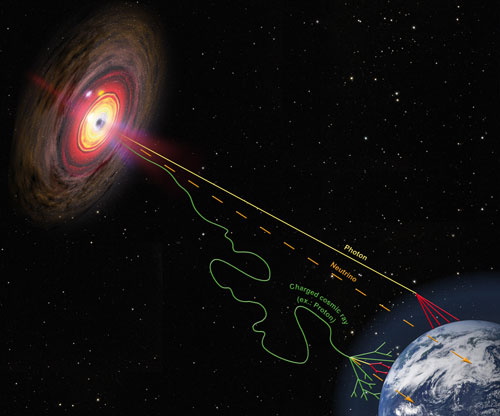
\includegraphics[width=9cm]{Plots/cosmic_ray.jpg}
    \caption{Charged and uncharged particles propagation through space}
    \label{fig:cosmic_ray}
\end{figure}

Gamma particles as well as hadrons can not cut through the earth's aerosphere and collide therefore with it.
Upon this collision the cosmic particle transfers some of its energy the its collision partner.
This causes an air shower by reason of the high energies of 0-0eV? involved.
Since the speed of light in air is lower than in space some air shower particles can be faster than the light speed in air
without violating the cosmic speed of light.
In this case those particles emit a cone of Tcherenkov radiation caused by the identically named effect.
When a high energetic cosmic particle interacts with the aerosphere, a short flash of Tcherenkov light can be detected at ground-level.

\begin{figure}
    \centering
    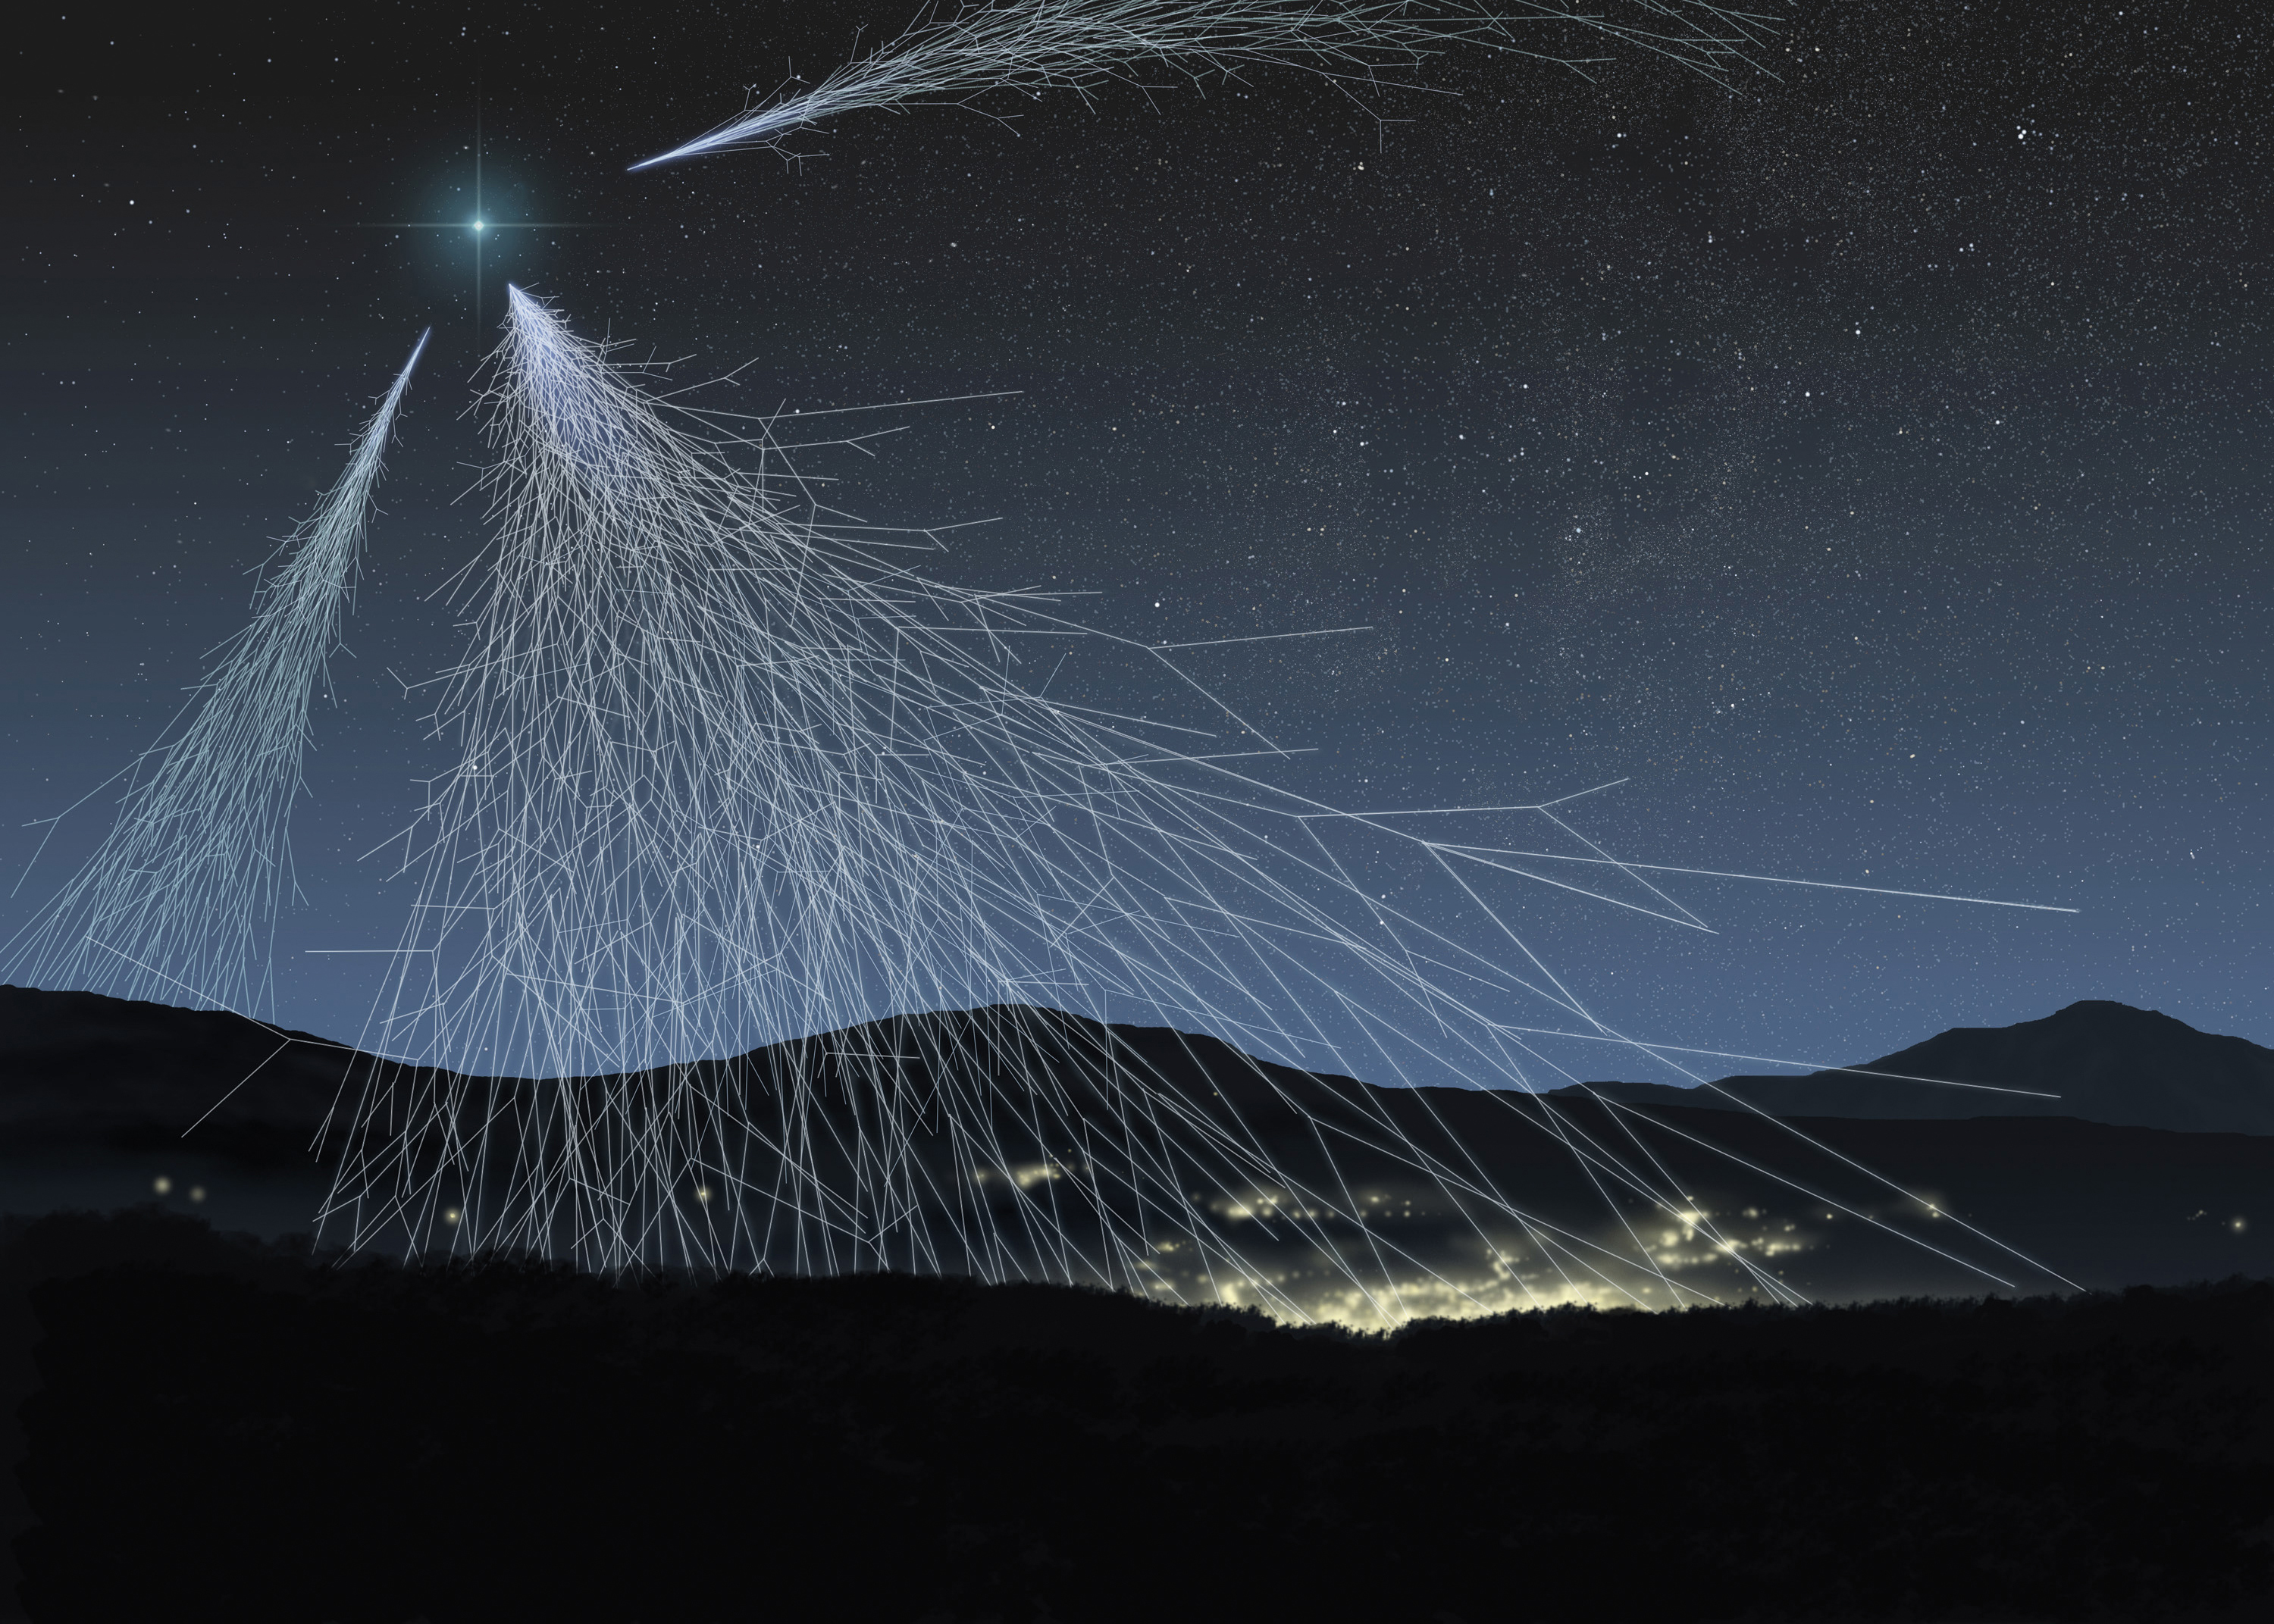
\includegraphics[width=9cm]{Plots/air_shower.jpg}
    \caption{Gamma ray causing an air shower in the aerosphere which emits Tcherenkov light}
    \label{fig:air_shower}
\end{figure}


\section{FACT telescope}
Among other telescopes the First G-APD Cherenkov Telescope (FACT) on La Palma records these light flashes.
It uses Geiger-mode avalanche photodiods (G-APDs) as photo sensors for a test benchmark of this technology.
With its small mirror surface of 9.5 sqm it operates since 2011
and collects data of air showers caused by cosmic radiation in the TeV energy range.

The 1440 camera pixel form a hexagonal grid.
This hexagonal pixel structure represents a challenge for the further image processing
since software for image classification was developed for images with quadratic pixels.
Therefor the camera image has to be transformed by using the pixel ids to map the hexagonal to a quadratic grid structure.
Skewing the image and padding it with empty pixels enables further processing without developing special software.
One drawback of this procedure is the loss of some direct neighborhood information
(hexagonal: 6 neighbors, quadratic: 4 neighbors) of every pixel.

\begin{figure}
    \centering
    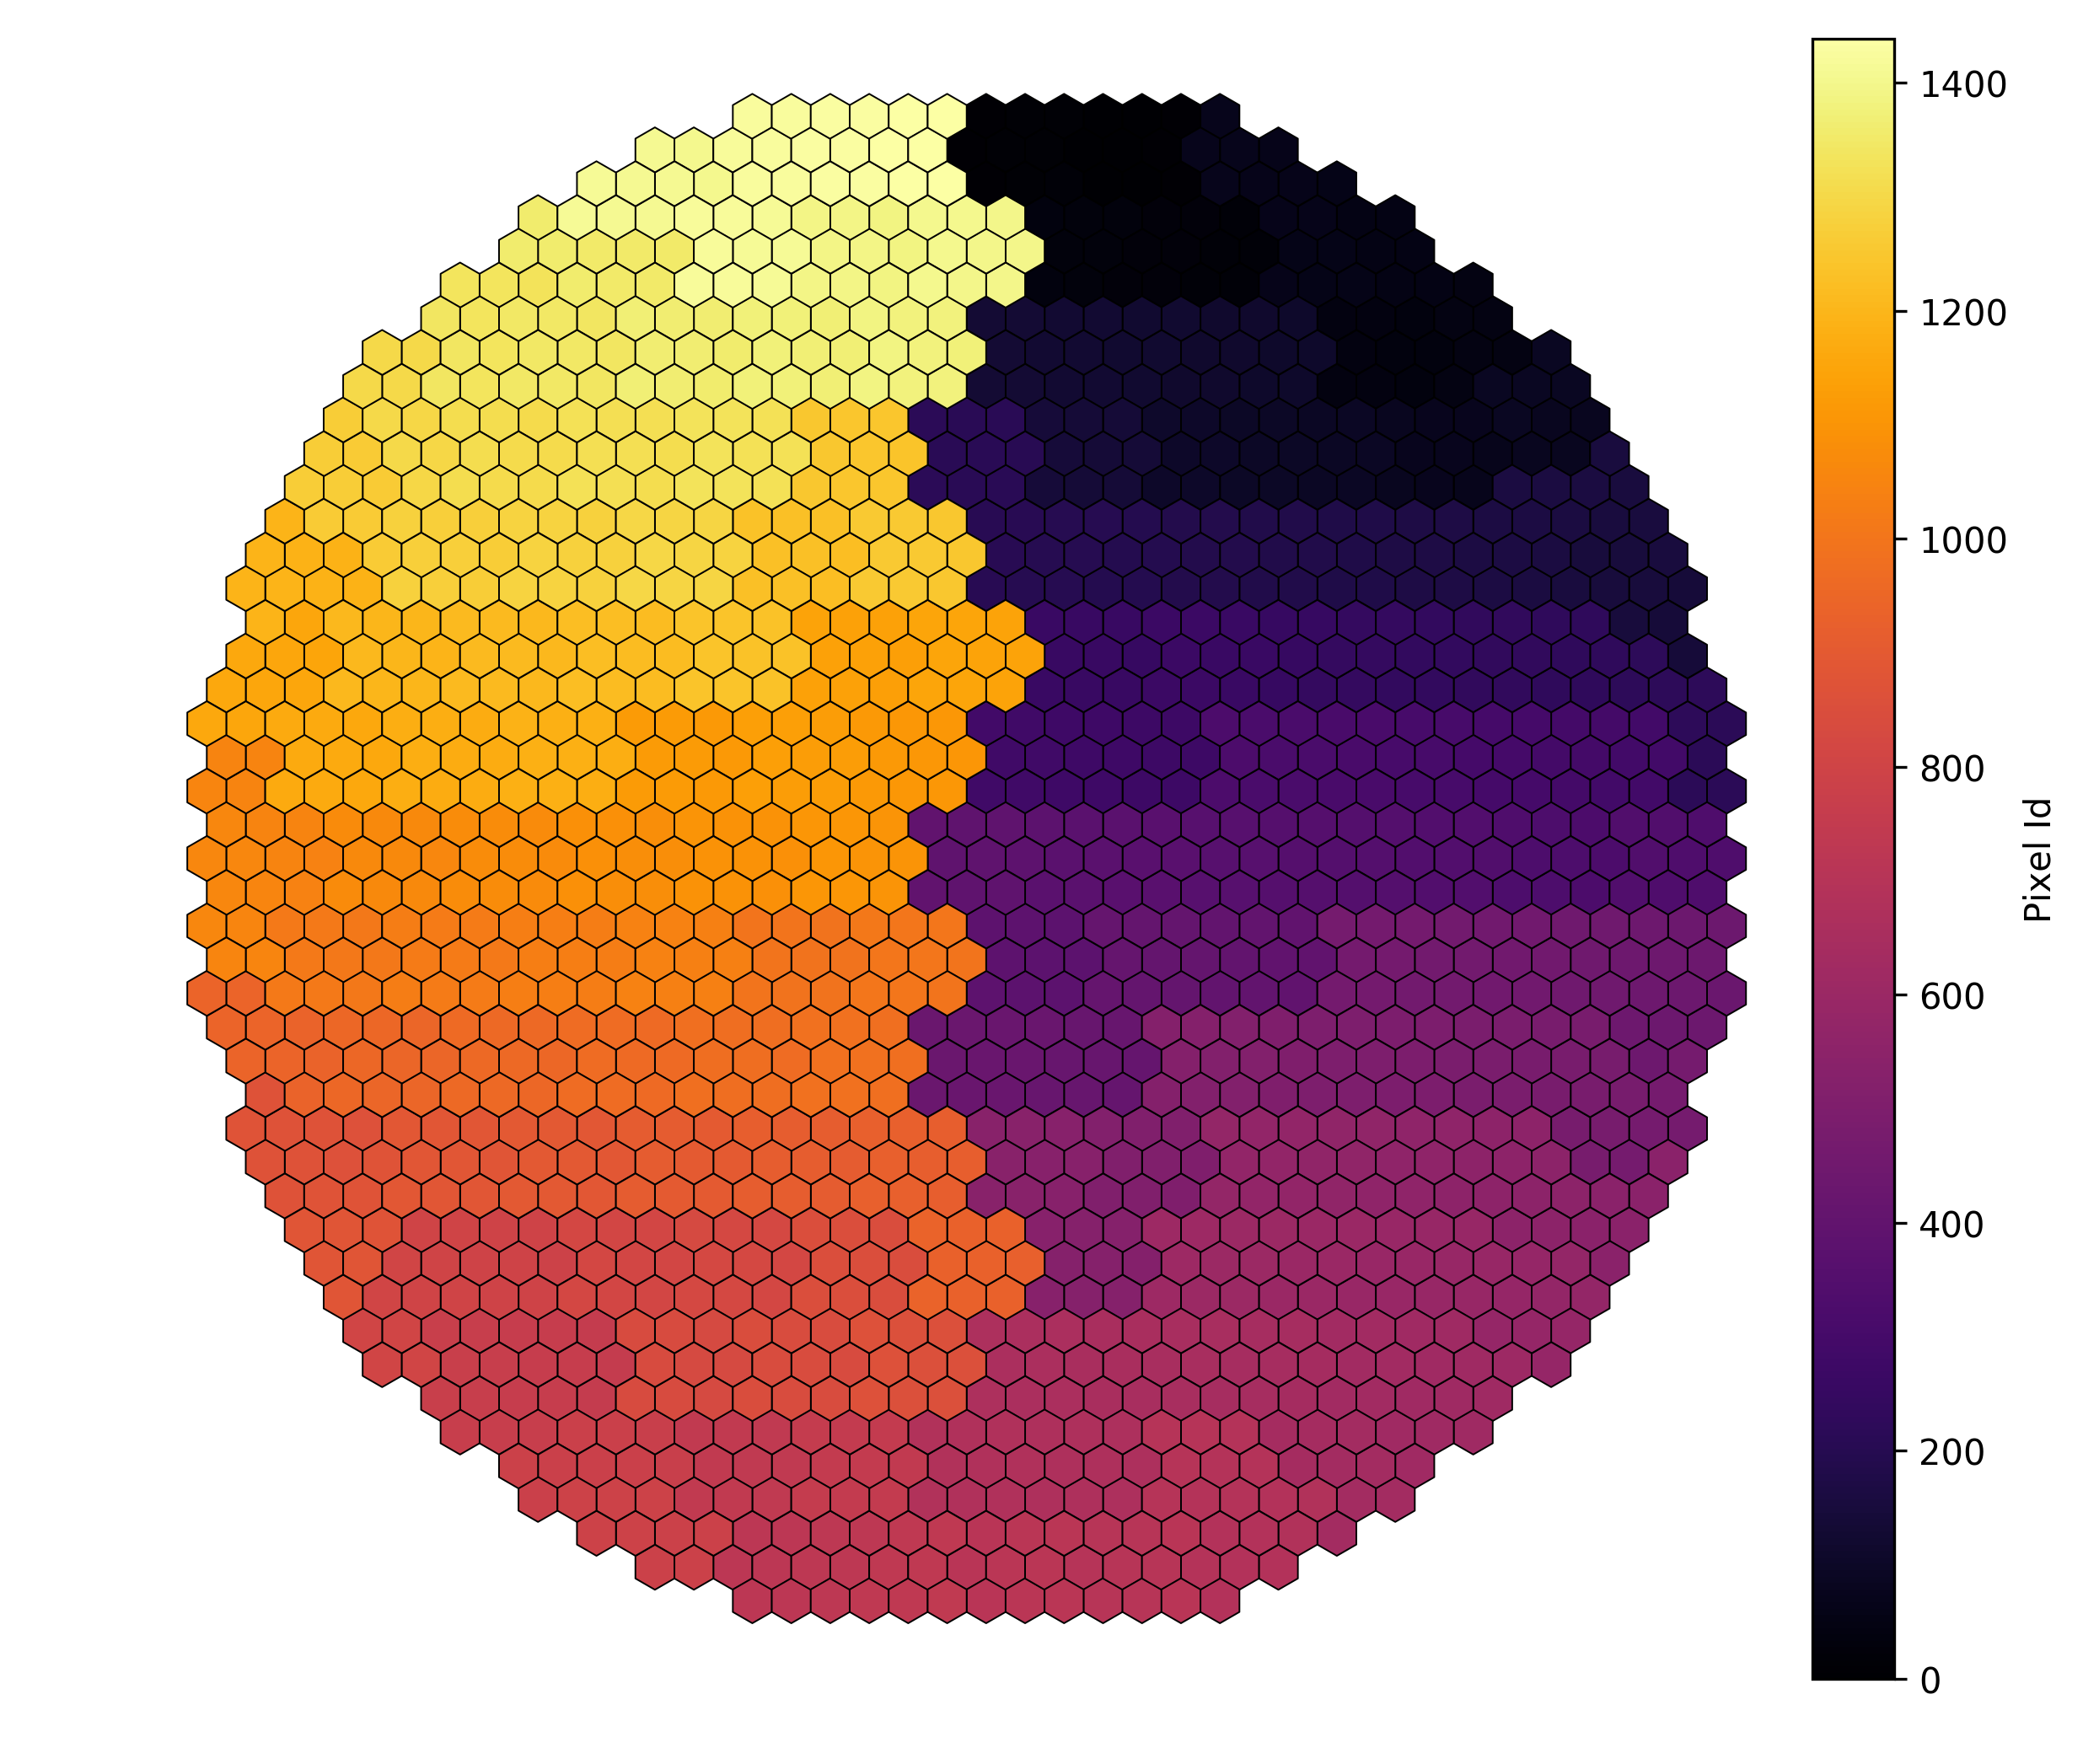
\includegraphics[width=6cm]{Plots/FACT_Image.png}
    \caption{FACT camera image with hexagonal pixels and the mapping axes}
    \label{fig:fact_image}
\end{figure}

\begin{figure}
    \centering
    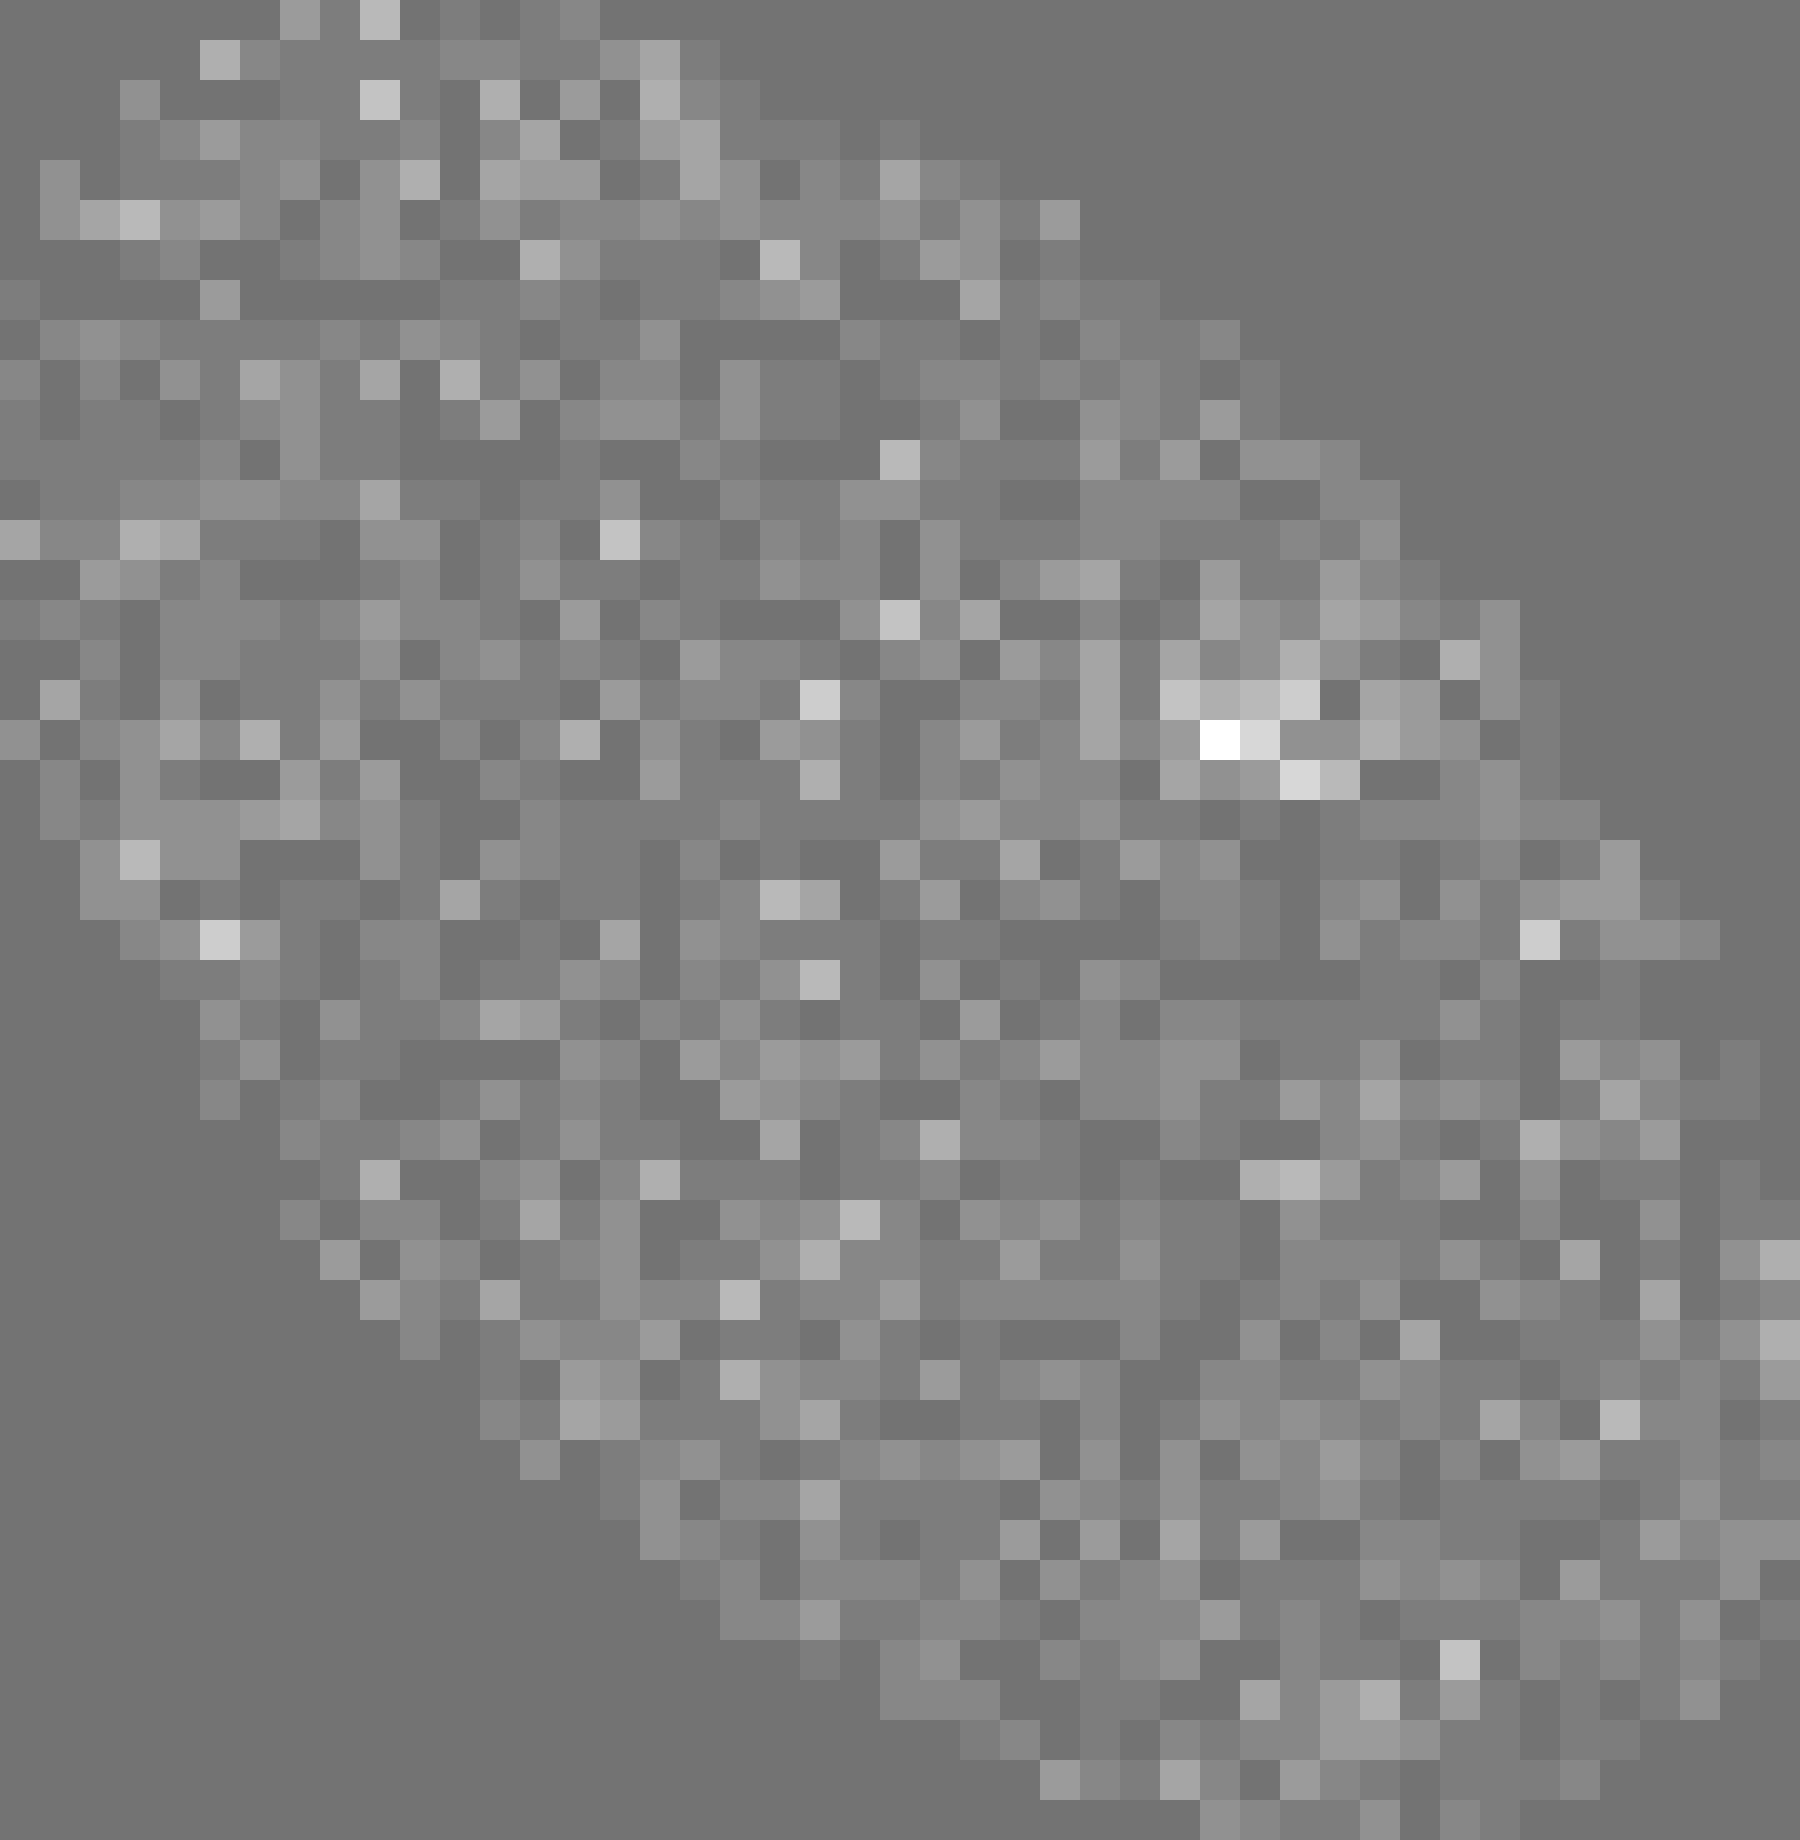
\includegraphics[width=6cm]{Plots/Preprocessed_Image.png}
    \caption{Skewed input image mapped to quadratic pixels}
    \label{fig:preprocessed_image}
\end{figure}



\section{Convolutional Neural Networks}
In the recent years Deep Learning evolved at an incredible rate and generated impressive progress in image classification tasks.
Utilizing the progress this thesis tests the benefit of Convolutional Neural Networks (CNN) for classifying the skewed camera images
by their triggering cosmic particle.
To separate images caused by gammas or hadrons there are many possible architectures for the CNN.
Every architecture is composed of layers with different tasks.
The image will then be passed and transformed from layer to layer till it reaches the last one.

Convolution layers (depicted in the plots as 'c') act as feature generators.
Patterns in the image will be translation invariant recognized.
Pooling layers reduce the feature space by selecting the most important ones.
They are following a convolution layer and will not be depicted in the plots.
Fully connected layers (depicted as 'f') complete the network in the final stages.
They combine the computed features and classify the image at the same time.

To minimize overfitting and maximize generalization different approaches can be used.
For evenly distributed pixel values batch normalization is used.
At the cost of longer training times Dropout layers ('d') can be inserted after any layer.
This will destroy some of the information flowing through the network
and force it to learn distributed representations of every feature making it more robust.
To enable long networks and faster training pretraining will be implemented.
After training small networks for a short time a new untrained layer will be attached.
This process will be iterated until the networks growth reached its final length.
While most of the layers only have to adapt slightly
the new layers can adjust their behaviour according the pretrained network quickly.

\begin{figure}
    \centering
    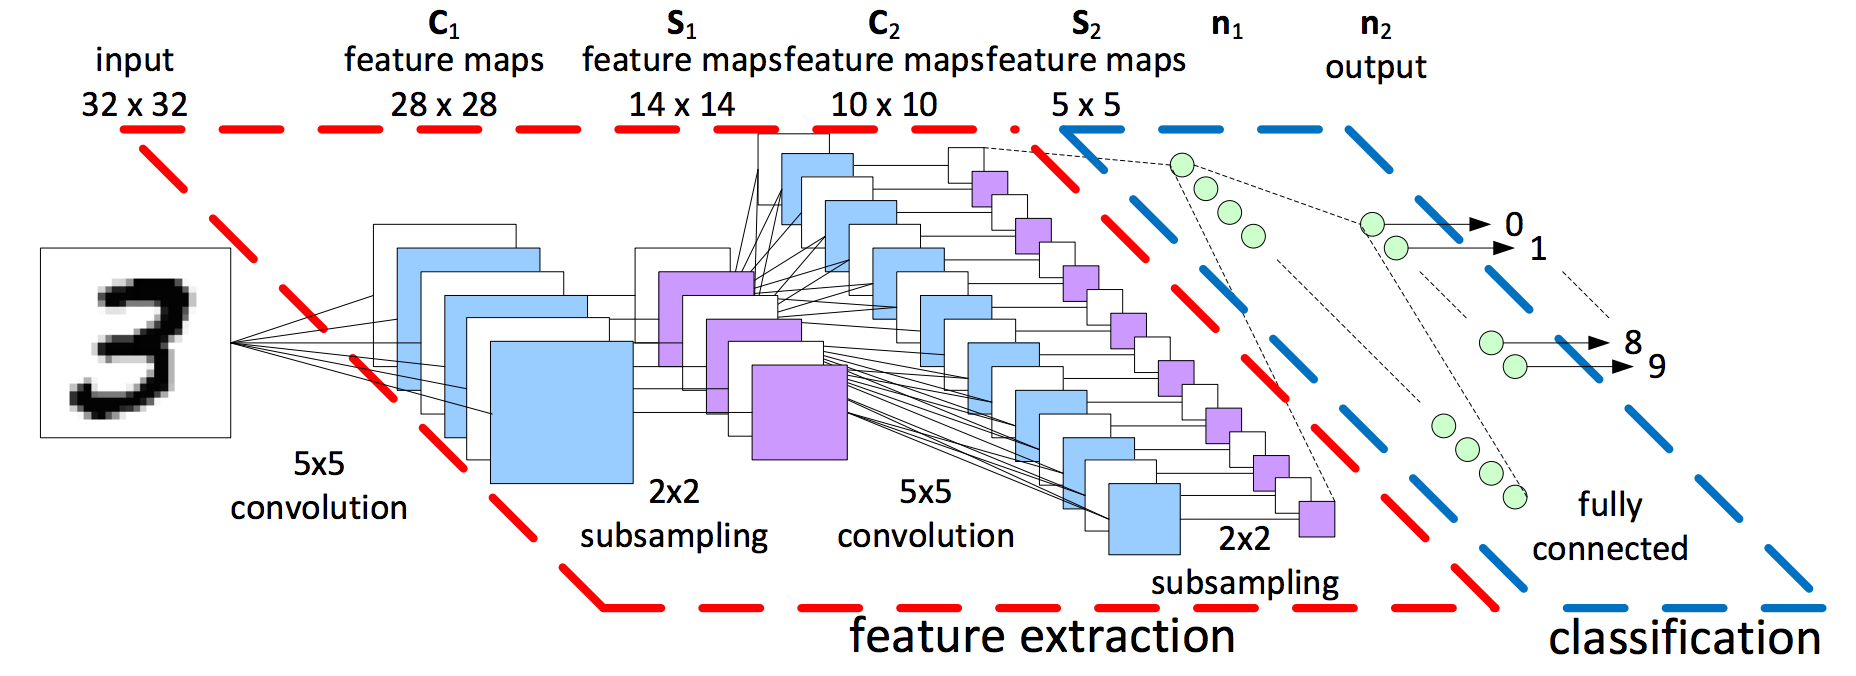
\includegraphics[width=12cm]{Plots/cnn_example.png}
    \caption{Example architecture of a CNN with Convolution, Pooling and Fully connected layers}
    \label{fig:cnn_example}
\end{figure}
